\begin{frame}{Why 3D Gaussian Splatting?}
    \justifying
    \vspace{0.5em}
    
    \begin{itemize}
        \justifying
        \item \textbf{The NeRF Dilemma} \\
        Neural Radiance Fields (NeRFs) are either slow and provide photorealistic scenes or they are reasonably fast but have to sacrifice image quality. Real-time applications are not possible.
        
        \vspace{1.5em}
        
        \item \textbf{3D Gaussians as a Novel Approach} \\
        Using 3D Gaussians as the differentiable, explicit base primitive, and abandoning neural networks was the key to unlocking previously unseen rendering speeds.
        
        \vspace{1.5em}
        
        \item \textbf{Impact on the field of 3D Reconstruction} \\
        Real-time rendering of reconstructed scenes represents a disruption in 3D Reconstruction enabling many new downstream applications.
    \end{itemize}
    \pdfcomment[opacity=0]{
        - 3D Gaussian Splatting is another technology in the field of 3D reconstruction\textCR
        - It takes its motivation directly from the shortcomings of neural radiance fields which Carmen presented just before\textCR
        - implicit vs explicit \textCR
        \textCR
        \textCR
        - Let's first look at the agenda. After a short background section, we'll start by examining the 3D Gaussian data structure before we dissect the training procedure in more detail. I'll finish by showing how the rendering process works, also called novel-view synthesis.\textCR
    }
\end{frame}

\section{Background}

% \begin{frame}{Background: From NeRFs to 3D Gaussians}
%     \begin{columns}[T]
%         % Left Column: Spotlighted Concepts
%         \begin{column}{0.35\textwidth}
%             \textbf{Evolution}
%             \vspace{1em}
            
%             \alt<1>{\textbf{\textcolor{blue}{The Rendering Challenge}}}{\textcolor{gray}{The Rendering Challenge}}\par\vspace{1em}
%             \alt<2>{\textbf{\textcolor{blue}{The 3DGS Solution}}}{\textcolor{gray}{The 3DGS Solution}}\par\vspace{1em}
%             \alt<3>{\textbf{\textcolor{blue}{Hardware \& Impact}}}{\textcolor{gray}{Hardware \& Impact}}
%         \end{column}

%         % Right Column: Synchronized Explanations
%         \begin{column}{0.6\textwidth}
%             \textbf{Key Concepts}
%             \vspace{1em}
            
%             \begin{overlayarea}{\textwidth}{5.5cm}
%                 \justifying
%                 \only<1>{
%                     \textbf{Novel-View Synthesis \& NeRFs}\\
%                     The goal is to generate new viewpoints from a set of 2D images. Prior methods like Neural Radiance Fields (NeRFs) rely on neural networks and \textit{volumetric ray marching}. \\
%                     \vspace{1em}
%                     This forces a strict trade-off: high photorealism requires slow rendering speeds or higher rendering speeds come with lower image quality.
%                 }
%                 \only<2>{
%                     \textbf{Explicit 3D Primitives}\\
%                     3D Gaussian Splatting (3DGS) abandons neural networks entirely. It explicitly models the scene using millions of differentiable 3D ellipsoids (``fuzzy blobs''). \\
%                     \vspace{1em}
%                     Instead of ray marching, these Gaussians are projected directly onto the 2D image plane via \textit{splatting}, bypassing previous computational bottlenecks.
%                 }
%                 \only<3>{
%                     \textbf{Real-Time Performance}\\
%                     By pairing explicit geometry with a highly optimized, tile-based GPU rasterizer, 3DGS achieves real-time rendering at 1080p (100+ FPS).\\
%                     \vspace{1em}
%                     Introduced in late 2023 by Kerbl et al., it disrupted 3D reconstruction by offering state-of-the-art visual quality alongside direct, immediate scene editability.
%                 }
%             \end{overlayarea}
%         \end{column}
%     \end{columns}
% \end{frame}

\begin{frame}{3D Reconstruction Terminology}
    \begin{columns}[T]
        % Left Column: Spotlighted Concepts
        \begin{column}{0.35\textwidth}
            \textbf{Core Concepts}
            \vspace{1em}
            
            \alt<1>{\textbf{\textcolor{blue}{3D Scene Creation}}}{\textcolor{gray}{3D Scene Creation}}\par\vspace{1em}
            \alt<2>{\textbf{\textcolor{blue}{Novel-View Synthesis}}}{\textcolor{gray}{Novel-View Synthesis}}\par\vspace{1em}
            %\alt<3>{\textbf{\textcolor{blue}{Radiance Field}}}{\textcolor{gray}{Radiance Field}}\par\vspace{1em}
            \alt<3>{\textbf{\textcolor{blue}{Splatting}}}{\textcolor{gray}{Splatting}}
        \end{column}

        % Right Column: Synchronized Explanations
        \begin{column}{0.6\textwidth}
            \textbf{Definitions}\\
            \vspace{1em}
            \begin{overlayarea}{\textwidth}{4cm}
                \justifying
                \only<1>{Creates 3D environments such as individual objects or outdoor spaces from an overlapping set of 2D input images.}
                \only<2>{Synthesizes new 2D imagery from the 3D scene using new camera positions.\\
                \vspace{1em}
                Real-time capability requires at least 24--30 frames per second (FPS) to appear smooth enough for the human eye.}
                %\only<3>{A function mapping coordinates and viewing angles to color and opacity at the given coordinates.\\Implicit fields are continuous; explicit fields use a finite set of points.}
                \only<3>{The process of moving all elements inside the view frustum onto the view plane preserving order, adding to aggregated color and opacity of each pixel.\\
                \vspace{2mm}
                \hspace*{3mm}
                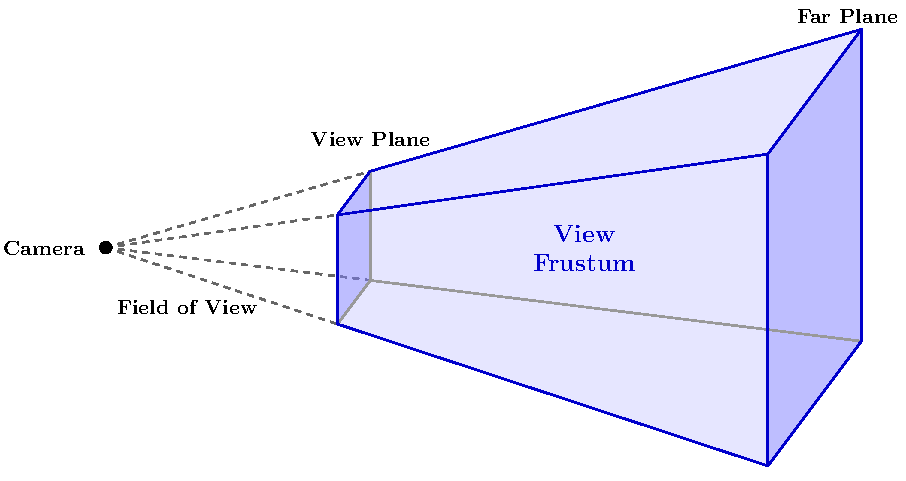
\includegraphics[width=0.88\textwidth]{../figures/view_frustum.pdf}
                }
            \end{overlayarea}
        \end{column}
    \end{columns}
    \pdfcomment[opacity=0]{
        - 3D Reconstruction is a field in Computer Graphics. It's basic components are scene creation .... and novel-view synthesis.\textCR
    }
    \only<3>{\pdfcomment[opacity=0]{
        - Splatting is in essence the reverse procedure to volumetric ray marching used in NeRFs.\textCR
        - Now let's continue with an overview of 3D Gaussian Splatting.\textCR
    }}
\end{frame}


% \begin{frame}{Neural Radiance Fields (NeRFs) as a Predecessor to 3D Gaussian Splatting}
%     \begin{columns}[T]
%         % Left Column: Spotlighted Concepts
%         \begin{column}{0.35\textwidth}
%             \textbf{Characteristics \& Limits}
%             \vspace{1em}
            
%             \alt<1>{\textbf{\textcolor{blue}{Implicit Representation}}}{\textcolor{gray}{Implicit Representation}}\par\vspace{1em}
%             \alt<2-3>{\textbf{\textcolor{blue}{Volumetric Ray Marching}}}{\textcolor{gray}{Volumetric Ray Marching}}\par\vspace{1em}
%             \alt<4>{\textbf{\textcolor{blue}{Training Bottlenecks}}}{\textcolor{gray}{Training Bottlenecks}}\par\vspace{1em}
%             \alt<5>{\textbf{\textcolor{blue}{``Black Box'' Inflexibility}}}{\textcolor{gray}{``Black Box'' Inflexibility}}\par\vspace{1em}
%             \alt<6>{\textbf{\textcolor{blue}{Quality vs. Speed}}}{\textcolor{gray}{Quality vs. Speed}}
%         \end{column}

%         % Right Column: Synchronized Explanations
%         \begin{column}{0.6\textwidth}
%             \textbf{Details}
%             \vspace{1em}
            
%             \begin{overlayarea}{\textwidth}{5.3cm}
%                 \justifying 
%                 \only<1>{
%                     NeRFs learn an implicit radiance field representation, meaning the full 3D scene is encoded entirely within the neural network's weights.
%                 }
%                 \only<2>{
%                     To synthesize novel views, NeRFs transmit a ray for every pixel, resulting in a very high number of queries to the neural network for discretized points along the ray's path.\vspace{1em}\\
%                     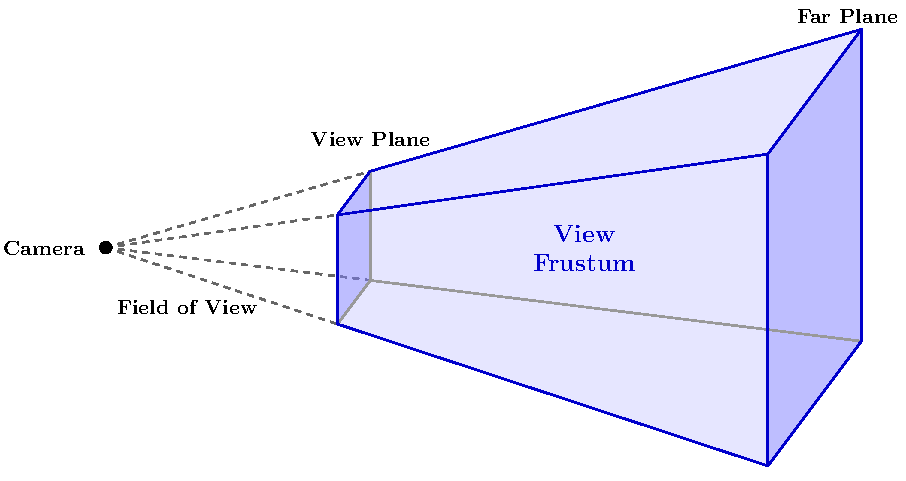
\includegraphics[width=0.8\textwidth]{../figures/view_frustum.pdf}
%                 }
%                 \only<3>{
%                     Ray marching and splatting are opposite ways to determine a pixel color value.
%                 }
%                 \only<4>{
%                     Training NeRFs to reach photorealistic scene quality can take several days on professional high-end GPU hardware.\\
%                     Ray marching during synthesis is highly time-con\-su\-ming.
%                 }
%                 \only<5>{
%                     Because all scene details are hidden inside the neural network's weights, it is not easily possible to edit or amend a reconstructed scene.
%                 }
%                 \only<6>{
%                     NeRFs force a trade-off: state-of-the-art reconstruction quality requires long training and synthesis times.\\Abandoning the neural network for explicit representations increases speed but inherently reduces image quality.
%                 }
%             \end{overlayarea}
%         \end{column}
%     \end{columns}
% \end{frame}


% \begin{frame}{3D Gaussian Splatting: Overview}
%     \begin{columns}[T]
%         % Left Column: Spotlighted Concepts
%         \begin{column}{0.35\textwidth}
%             \textbf{Core Innovations}
%             \vspace{1em}
            
%             \alt<1>{\textbf{\textcolor{blue}{Origin \& Architecture}}}{\textcolor{gray}{Origin \& Architecture}}\par\vspace{1em}
%             \alt<2>{\textbf{\textcolor{blue}{The Base Primitive}}}{\textcolor{gray}{The Base Primitive}}\par\vspace{1em}
%             \alt<3>{\textbf{\textcolor{blue}{Fully Differentiable}}}{\textcolor{gray}{Fully Differentiable}}\par\vspace{1em}            
%             % \alt<4>{\textbf{\textcolor{blue}{Direct Editability}}}{\textcolor{gray}{Direct Editability}}\par\vspace{1em}
%             \alt<4>{\textbf{\textcolor{blue}{Hardware Optimization}}}{\textcolor{gray}{Hardware Optimization}}
%         \end{column}

%         % Right Column: Synchronized Explanations
%         \begin{column}{0.6\textwidth}
%             \justifying 
%             \textbf{Details}
%             \vspace{1em}
            
%             \begin{overlayarea}{\textwidth}{4.3cm}
%                 \justifying
%                 \only<1>{
%                     Introduced by Kerbl et al. at INRIA in France in late 2023, 3D Gaussian Splatting (3DGS) combines existing concepts to create a learnable explicit radiance field representation.\\
%                     \vspace{1em}
%                     The publication had a very high impact in the field with over 10,000 citations in three years.
%                 }
%                 \only<2>{
%                     A 3D Gaussian is an ellipsoid ``fuzzy blob'' that loses opacity towards its edges and can take shapes ranging from perfect spheres to elongated needles or flat shapes.\\
%                     \vspace{1em}
%                     Using them as base primitives bypasses previous issues with explicit fields and allows for arbitrary positional precision.
%                 }
%                 \only<3>{
%                     Using clever decompositions of 3D Gaussians, they become differentiable and eligible for standard gradient descent backpropagation.\\
%                     \vspace{1em}
%                     Most importantly, this means 3DGS operates completely without neural networks which removes the ``blackbox'' associated with them.
%                 }
%                 % \only<4>{
%                 %     Unlike the neural network ``black box'' of NeRFs, 3D Gaussians provide direct editability of the scene.\\
%                 %     \vspace{1em}
%                 %     This makes scene modifications, such as additions or lighting changes, highly accessible for downstream applications.
%                 % }
%                 \only<4>{
%                     Kerbl et al. mapped their architecture exhaustively onto modern GPU hardware.\\
%                     \vspace{1em}
%                     The centerpiece is the tile-based rasterizer, which allows real-time novel-view synthesis at 1080p resolution while matching or improving upon state-of-the-art NeRF quality.
%                 }
%                 \only<3>{\pdfcomment[opacity=0]{
%                     - Editability, extensibility
%                 }}
%                 \only<4>{\pdfcomment[opacity=0]{
%                     - For the engineering side of the publication...\textCR
%                     \textCR
%                     - Now that we know what 3DGS is in broad terms, let's have a look at what a 3D Gaussian or a Gaussian in general is.
%                 }}
%             \end{overlayarea}
%         \end{column}
%     \end{columns}
% \end{frame}